% Preamble
\documentclass[11pt]{PyRollDocs}

\addbibresource{refs.bib}

% Document
\begin{document}

    \title{The Stationary Thermal Analysis Work Roll PyRolL Plugin}
    \author{Christoph Renzing}
    \date{\today}

    \maketitle


    \section{Model approach}\label{sec:model-approach}

    The PyRolL plugin is based on the paper of \textcite{Robinson1996}, and enables the calculation of the 2D - Temperature Field inside a Work Roll witch is subjected to cooling (e.g.~Water Cooling) as well as heat transfer (e.g.~Inside the roll gap or through contact with supporting rolls.)
    Using this model, the surface temperature along the radius of the roll can be calculated by solving the differential equation for this two-dimensional steady state using non-rotating coordinates.

    \begin{equation}
        \nabla_2^2 T = \left( \frac{\partial^2}{\partial r^2} + \frac{1}{r}\frac{\partial}{\partial r} + \frac{1}{r^2}\frac{\partial^2}{\partial \theta^2} \right) T = \frac{1}{Pe^2}\frac{\partial T}{\partial \theta}
        \label{eq:1}
    \end{equation}


    In this equation, $\theta$ is the angular coordinate and $r$ is the radius.
    Further the author noted, that using non-dimensional quantities eases up dealing with numerical difficulties.
    Therefore, the radius as well as other important variables will be made non-dimensional accordingly.
    In General, the differential equation can be solved using Fourier analysis.
    \textcite{Patula1981}  derived the following equation from the original ODE.


    \begin{equation}
        T = \sum_{n=-\infty}^{n=\infty} A_n \cdot F_n(r) \exp\left(i \cdot n \cdot \theta \right)
        \label{eq:2}
    \end{equation}


    The roll is heated due to the profiles temperature, during the same moment, it is cooled using a water spray cooling.
    The following \autoref{fig:1} shows the classic water cooling arrangement for a roll used in a wire rod block.
    The angles $\theta_1$ and $\theta_2$ represent the initial and finishing angle of the cooling, counted counterclockwise.

    \begin{figure}
        \centering
        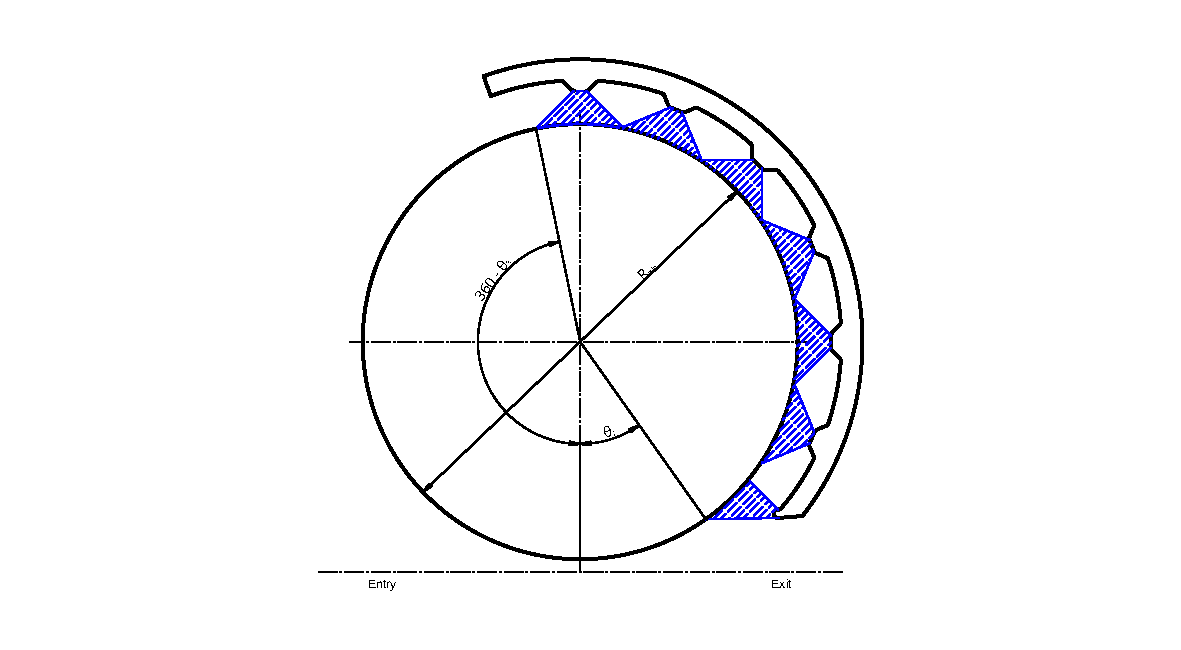
\includegraphics[width=\textwidth]{img/cooling_finishing_block}
        \caption{Schematic Cooling of a roll operating inside a wire rod finishing rod.}
        \label{fig:1}
    \end{figure}

    To further analyse the problem, we need to express the cooling as well as heating function as a fourier series.
    Therefore, we need to calculate the fourier coefficients according to the following equations:

    \begin{equation}
        H_n = \frac{1}{2 \pi} \int_{0}^{2 \pi} h_{nor}(\theta) \exp\left( -i \cdot n \cdot \theta \right)d\theta
        \label{eq:3}
    \end{equation}

    \begin{equation}
        Q_n = \frac{1}{2 \pi} \int_{0}^{2 \pi} q_{nor}(\theta) \exp\left( -i \cdot n \cdot \theta \right)d\theta
        \label{eq:4}
    \end{equation}

    \subsection*{Calculation of Fourier Terms for Temperature Calculation}
    Further we have to calculate the Fourier Coefficients for the solution of the Temperature field proposed by \textcite{Patula1981}.

    \begin{equation}
        T = \sum_{n=-\infty}^{n=\infty} A_n \cdot F_n(r*) \exp\left(i \cdot n \cdot \theta \right)
        \label{eq:5}
    \end{equation}

    The Fourier Term $F_n$ is calculated using the formula:

    \begin{equation}
        F_n(r*) = \frac{J_n\left( \sqrt{-i \cdot n} \frac{r*}{\epsilon}\right)}{J_n\left( \sqrt{-i \cdot n} \frac{1}{\epsilon}\right)}
        \label{eq:6}
    \end{equation}

    In this equation $J_n$ is the n-th order Bessel function of the first kind.
    Norming the values of the Bessel function $J_n$ using the values at the surface ($r* = 1$) is necessary since for large orders $n$ the value of the Bessel function can exceed values of $10^{5000}$.
    To further handel such big numbers, inside the code, we use the package \emph{mpmath} witch allows for high precision calculations and can easily handel larger numbers.

    \subsection*{Calculation of Fourier Coefficients $A_n$}
    Next up, we need to calculate the Fourier coefficients matrix $A_n$.
    The values of this matrix are solely dependent on from the boundary condition at the surface of the roll.
    At the surface ($r^* = 1$), we have the following boundary condition of Robin type:

    \begin{equation}
        \frac{dT^*}{dr^*} = -h^*(\theta) + q^*(\theta)
        \label{eq:7}
    \end{equation}

    If we insert the Fourier series for $h^*$ and $q^*$ accordingly and see that due to the normalisation of $F_n$ it's values become 1 for all orders n at the surface.
    So the following equation results from this:

    \begin{equation}
        A_n \frac{dF_n}{dr^*} (1) + \sum_{m=-\infty}^{m=\infty} H_{n-m}A_m = Q_n
        \label{eq:8}
    \end{equation}

    for the order n being $0, \pm 1, \pm 2, \ldots$.

    In matrix form this equation can be expressed as: $k_n^{-1}A_n = Q_n$ or $A_n = k_nQ_n$.

    The invers matrix $k_n^{-1}$ calculated as follows (Example for N = 2):
    \begin{equation}
        k_n^{-1} =
        \begin{bmatrix}
            F'_{-2}(1) &            &   &           &           \\
            & F'_{-1}(1) &   &           &           \\
            &            & 0 &           &           \\
            &            &   & F'_{1}(1) &           \\
            &            &   &           & F'_{2}(1)
        \end{bmatrix}
        +
        \begin{bmatrix}
            H_0   & H_{-1} & H_{-2} &        &        \\
            H_{1} & H_0    & H_{-1} & H_{-2} &        \\
            H_{2} & H_{1}  & H_0    & H_{-1} & H_{-2} \\
            & H_{2}  & H_{1}  & H_0    & H_{-1} \\
            &        & H_{2}  & H_{1}  & H_0    \\
        \end{bmatrix}
        = F'_n + H_n
        \label{eq:9}
    \end{equation}

    To calculate der derivate $F'_n(r^*) = \frac{d}{dr^*} F_n(r^*)$ we use the following formula while building the derivate using the chain rule:

    \begin{equation}
        F_n'(r^*) = \frac{\sqrt{-i n}}{Pe} \cdot \frac{\frac{1}{2} \left(J_{n-1} \left( \sqrt{-i n} \frac{r^*}{Pe} \right) - J_{n+1} \left( \sqrt{-i n} \frac{r^*}{Pe} \right) \right)}
        {J_n \left( \sqrt{-i n} \frac{1}{Pe} \right)}
        \label{eq:10}
    \end{equation}

    \subsection*{Calculation of Derivates and Building Diagonal Matrix}
    At first, we calculate the derivates $F'_n(r^*)$ for this we again use the package `mpmath`.
    Next up we will build the diagonal matrix using the results.

    \subsection*{Calculation of the Invers Matrix $k_n^{-1}$}
    Using addition, the invers matrix $k_n^{-1}$ is calculated using the following equation.
    \begin{equation}
        k_n^{-1} = F'_n + H_n
        \label{eq:11}
    \end{equation}

    Further, we invers the matrix $k_n^{-1}$ to calculate the missing coefficients.
    Finally, we can calculate the matrix $A_n$.
    
    \begin{equation}
        A_N = k_n \cdot H_n
        \label{eq:12}
    \end{equation}
    
    To solve for the temperatures, we now evaluate \autoref{eq:2} for every angle.

    \section{Usage instructions}\label{sec:usage-instructions}
    
    The plugin defines certain hooks inside the \emph{Roll} class witch needs to be set.
    These are:
    \begin{itemize}
        \item \emph{specific\_heat\_capacity} - Specific heat capacity of the roll material
        \item \emph{thermal\_conductivity} - Thermal conductivity of the roll material
        \item \emph{density} - Density of the roll material
        \item \emph{cooling\_sections} - Cooling section angles $\theta$ as a List of Lists of start and stop angle.
        \item \emph{coolant\_heat\_transfer\_coefficient} - Heat transfer coefficient of the spray cooling [default: 15000 $\frac{W}{m^2 K}$]
        \item \emph{coolant\_temperature} - Temperature of the coolant [default: 308.15K]
        \item \emph{free\_surface\_heat\_transfer\_coefficient} - Heat transfer coefficient of the free surface[default: 15 $\frac{W}{m^2 K}$]
        \item \emph{heat\_transfer\_coefficient} - Heat transfer coefficient of the roll contact[default: 6000 $\frac{W}{m^2 K}$]
    \end{itemize}



    \printbibliography

\end{document}